\chapter{Ανάλυση και σχεδίαση}
\InitialCharacter{Σ}το κεφάλαιο αυτό παρουσιάζεται η μελέτη που έγινε για την υλοποίηση του συστήματος. Αρχικά περιγράφεται η αρχιτεκτονική του
συστήματος και γίνεται ο διαχωρισμός του στα επιμέρους
υποσυστήματα, ενώ στη συνέχεια περιγράφονται οι εφαρμογές του
συστήματος.

\section{Ανάλυση - περιγραφή αρχιτεκτονικής}
Στην ενότητα αυτή παρουσιάζεται η ανάλυση του συστήματος και ο
χωρισμός του σε υποσυστήματα όσον αφορά την αρχιτεκτονική.

\subsection{Διαχωρισμός υποσυστημάτων}
Το σύστημα αποτελείται από τους απλούς κόμβους και ένα κόμβο
διαχειριστή. Στο σημείο αυτό αναλύουμε το σύστημα ενός απλού
κόμβου, το οποίο αποτελείται από τα εξής υποσυστήματα:

\begin{itemize}
\item Υποσύστημα δημιουργίας σχήματος.
\item Υποσύστημα ενσωμάτωσης δεδομένων στο σχήμα.
\item Υποσύστημα επικοινωνίας κόμβου.
\end{itemize}

\begin{figure}[!ht] \centering
	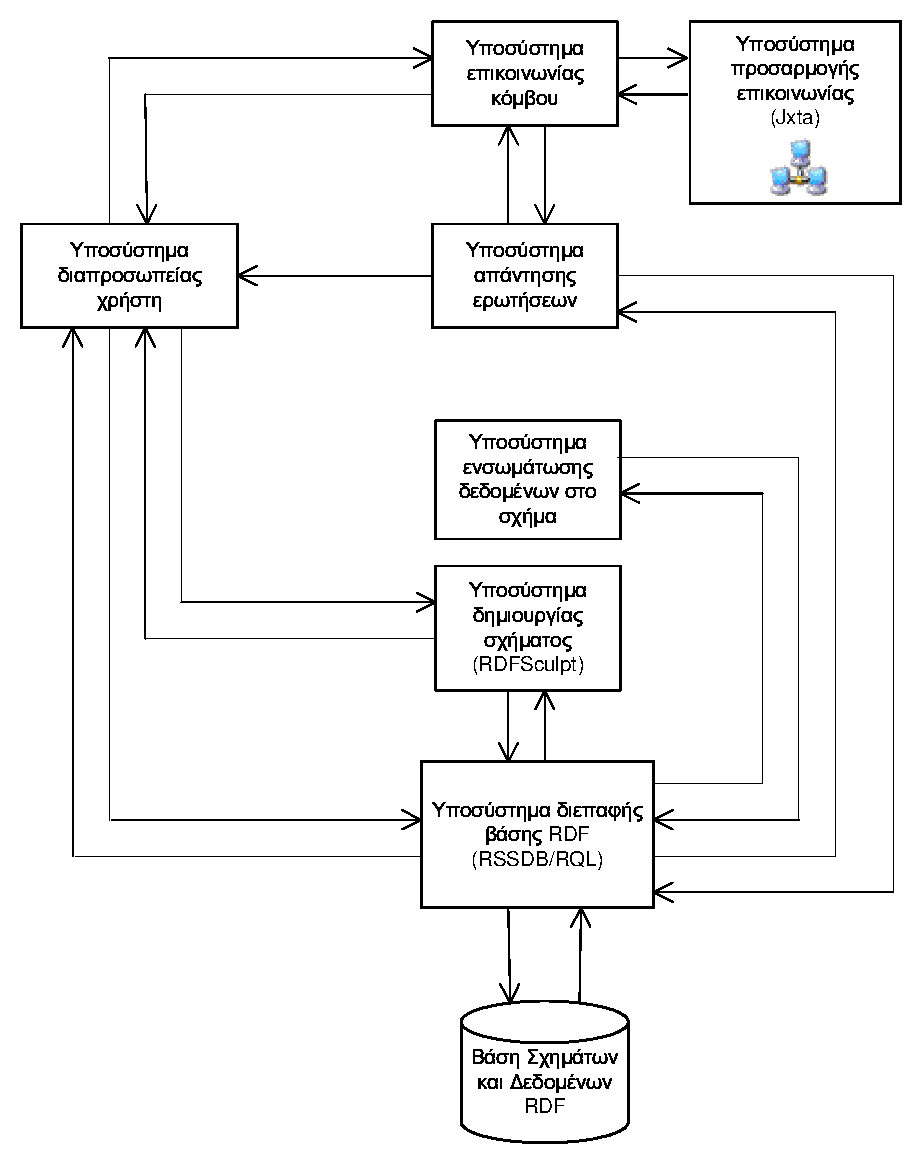
\includegraphics{figures/peerArchitecture.eps} 
    \caption{Αρχιτεκτονική Απλού Κόμβου}
    \label{figure4.1}
\end{figure} 

Το Σχήμα~\ref{figure4.1} απεικονίζει ..............


\subsection{Περιγραφή υποσυστημάτων}
Παρακάτω δίνεται λεπτομερής περιγραφή για καθένα από τα συστήματα
που αναφέραμε. Η περιγραφή αυτή γίνεται με βάση τα διαγράμματα
ροής δεδομένων.

\subsubsection{Υποσύστημα δημιουργίας σχήματος}
Το υποσύστημα αυτό ...............